\documentclass{beamer}

\usepackage[british]{babel}
\usepackage{graphicx,hyperref,tue,url}
\usepackage{amsmath}
\usepackage{xcolor}
% The title of the presentation:
%  - first a short version which is visible at the bottom of each slide;
%  - second the full title shown on the title slide;
\title[Network\_science]{
  Link Prediction:\\ 
  Similarity Indexes}
  %What is it and how to tackle it? }

%\subtitle{Similarity Indexes}

% The author(s) of the presentation:
%  - again first a short version to be displayed at the bottom;
%  - next the full list of authors, which may include contact information;
\author[Andrea Mangrella]{
  Andrea Mangrella\\
  Roëlle Bänffer\\
  Maarten van Sluijs\\
  }

% The institute:
%  - to start the name of the university as displayed on the top of each slide
%    this can be adjusted such that you can also create a Dutch version
%  - next the institute information as displayed on the title slide
\institute[Eindhoven University of Technology]{
  Department of Mathematics and Computer Science \\
  Eindhoven University of Technology}

% Add a date and possibly the name of the event to the slides
%  - again first a short version to be shown at the bottom of each slide
%  - second the full date and event name for the title slide
\date[slides Example 2012]{
    19th October 2023   
  }

\begin{document}

\begin{frame}
  \titlepage
\end{frame}

\begin{frame}
  \frametitle{Outline}
  \tableofcontents
\end{frame}

% INTRODUCTION:
\section{Introduction}
\begin{frame}
  \frametitle{Dataset: Jazz musicians}
  For this project, we will analyse the Jazz musicians dataset collected in 2013:\\
  We have a collaboration network between Jazz musicians. Each node is a band and each edge denotes a collaboration between bands. The bands are connected if they have a musician in common. \\
  We have 198 vertices and 2742 edges.
 
\begin{figure}
\centering
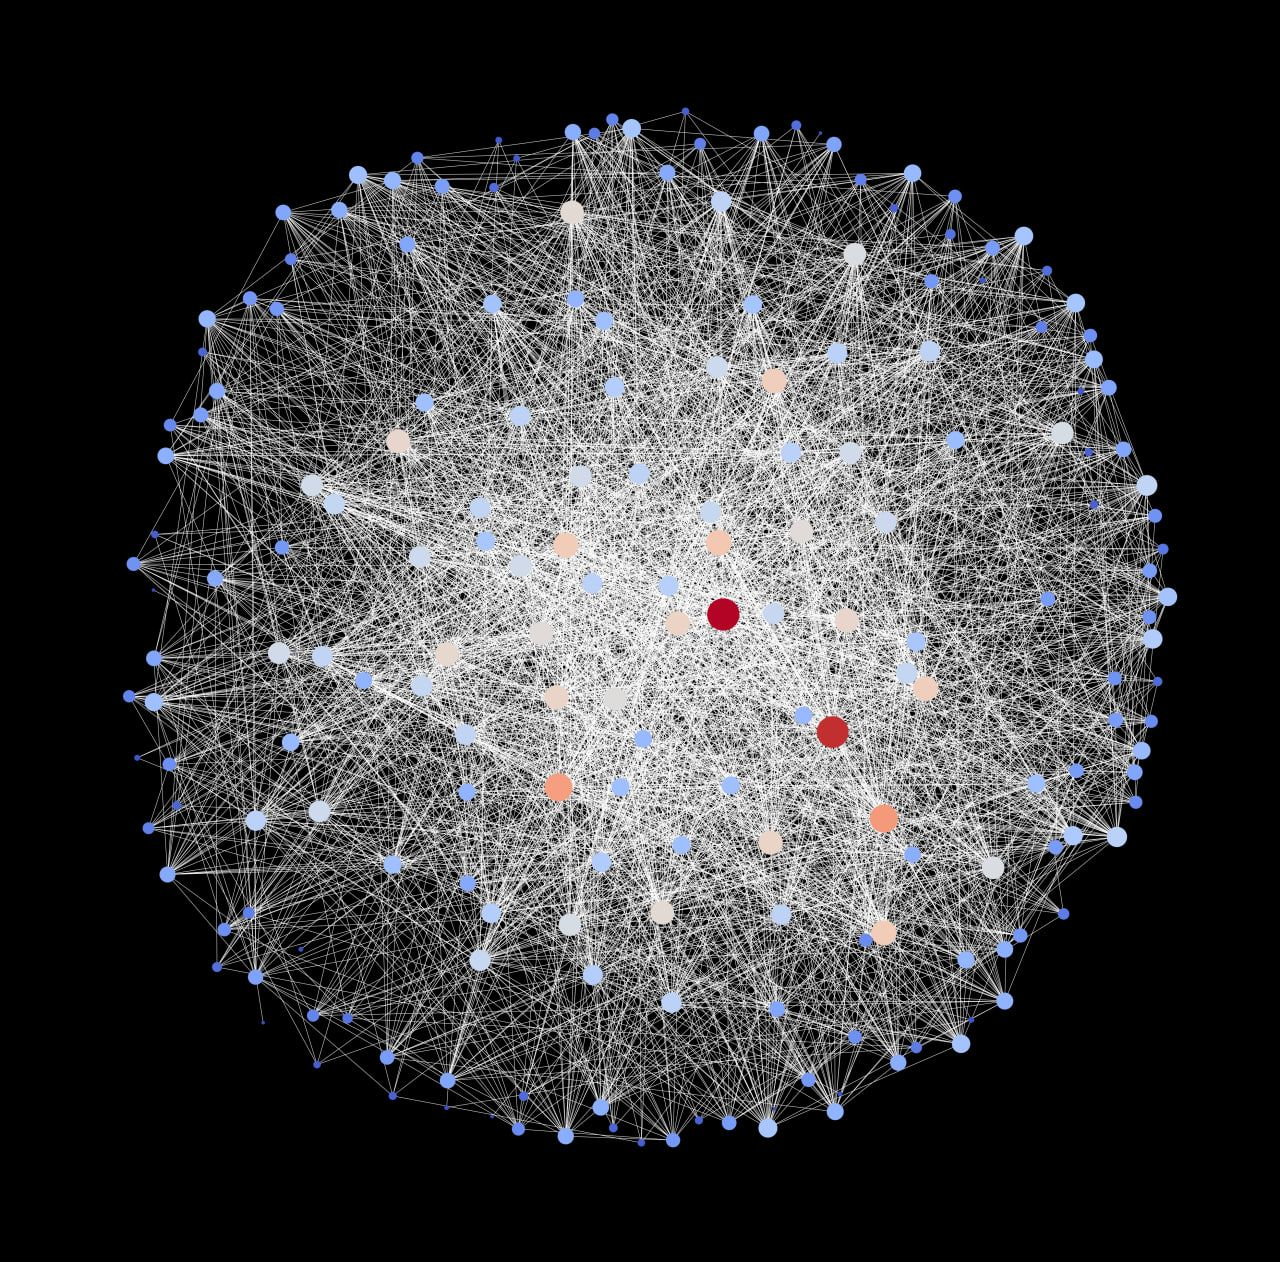
\includegraphics[width=.4\linewidth]{jazz_net.jpeg}
  \label{fig:jazz_net}
\end{figure}
 
\end{frame}

\begin{frame}
  \frametitle{Community structure in Jazz}
  \textbf{A common property of collaboration networks}:\\ Small world property is the average distance between vertices is small, while the clustering vertices remains high. (degree distribution P(k) is skewed)\\

  The dataset contains musicians that are unknown which could be different people. The goal is to detect these \textit{spurious links} (unknown musicians).\\
  

  \textbf{Spurious links detection}: \\
  Predict whether an association between the nodes present in the current state of the graph is spurious (should not exist)
  

  % Idea: Communities appear in networks where vertices join together in tight groups that have few connections between them. We isolate the communities by eliminating the connections between the communities.
  
\end{frame}

\begin{frame}
 \frametitle{Removing unknown links}
    Algorithm steps:
    \begin{itemize}
        \item Find the biggest clique in the graph
        \item Remove the internal edges of the biggest clique
        \item Using existing (dis) similarity indices to find a spurious link
        \item Compare different similarity indices
    \end{itemize}
Chosen existing similarity methods: \\
Local: Resource Allocation Index,\\
Global: Leicht-Holme-Newman Index
\end{frame}

% If there are more short paths between two vertices than expected, then there is probably also a direct path


% \begin{frame}
%  \frametitle{Applying existing method Leicht-Holme-Newman index }
%     \[D^{-1}*(I - \frac{\phi A}{\lambda_1})^{-1}*D^{-1}\]
% \end{frame}

\section{Testing and Metrics}
% \begin{frame}
%   \frametitle{Testing the Indices}
% To test the algorithm’s \textbf{Accuracy}, the observed links, E, are randomly divided into two parts: the \textbf{Training set} and the \textbf{Probe set}. \\%(\bold{E^T} and   \bold{E^P}). 
% \smallskip
% \color{purple}Disadvantage: \color{black} some link may \textbf{never be selected} in the probe set, and other may be selected many times.
% \end{frame}

% \begin{frame}
%   \frametitle{Testing the Indices}
% To test the algorithm’s \textbf{Accuracy}, the observed links, E, are randomly divided into two parts: the \textbf{Training set} and the \textbf{Probe set}. \\%(\bold{E^T} and   \bold{E^P}). 
% \smallskip
% \color{purple}Disadvantage: \color{black} some link may \textbf{never be selected} in the probe set, and other may be selected many times.\\
% \medskip
% \color{teal}Solution: \color{black} use k-cross validation, in which the edges get partitioned in \textbf{k} subset. The process is repeated k times to use \emph{\textbf{every subset as the probe set}}.
% \end{frame}
\begin{frame}
  \frametitle{Testing Metrics}
  \emph{\textbf{Accuracy}}: is the ratio of relevant items
to the number of selected item. The result unfortunately focuses only on the top L candidates\\
    \[Precision = \dfrac{l}{L}\] \\
  \bigskip 
  \emph{\textbf{AUC}}: the probability that a randomly chosen missing link (a link in EP) is given a higher score than a randomly chosen nonexistent link.The result is the overall ranking resulted from the algorithm. \\
   \[AUC = \dfrac{n' + 0.5n''}{n}\]
\end{frame}

\section{Our Index}
% \begin{frame}
% \frametitle{Comparison Index}
% \textbf{Resource Allocation Index:} \\
% \vspace{0.3cm}
% A Local index that is not just a variation of Common Neighbours. But considers the degree of the nodes that are part of \textbf{intersection of the 2 neighbourhoods}.\\
% Based on \textbf{resource allocations dynamics on Complex networks.} \\
% \vspace{0.2cm}
% \begin{align*}
% s^{RA}_{xy} = \sum_{z\in\Gamma_{x} \cap \Gamma_{y}}^{} \dfrac{1}{k_{z}}
% \end{align*}
% \vspace{0.2cm}
% \end{frame}

\begin{frame}
\textbf{Spectrum of the Laplacian:} \\
\vspace{0.6cm}
\color{teal}Idea:\color{black} \\
We suppose that in a social network graph the \textbf{likeliness that two nodes in the same community are connected} is much higher than the one between two nodes of different communities. \\
\vspace{0.2cm}
We wanted to \textbf{exploit the community structure} of the graph to get how likely two nodes are in the same community, and then use this value as a similarity index. \\ 
\end{frame}

\begin{frame}
\textbf{Similarity in The spectrum:} \\
We also used this index to find if an edge inside the clique is spurious or not:\\
The \textbf{lower} a value for an edge in the biggest clique, \textbf{the more likely that the edge is spurious.}
We used the L2 norm as a metric for distance between the eigenvectors of the 2 nodes.\\
\vspace{0.2cm}
\begin{align*}
s^{SS}_{xy} = \dfrac{1}{\sqrt{\sum_{k=1}^{n} (v^{x}_{k}-v^{y}_{k})^{2} }}
\end{align*}
\end{frame}

\section{Comparing our results}
\begin{frame}{LHN index vs Spectral index}
    \begin{table}[]
        \centering
        \begin{tabular}{llllll}
            \hline
            \multicolumn{3}{c|}{LHN} & \multicolumn{3}{|c}{Spectral}\\
            \hline
            Edge & Value & Path & Edge & Value & Path\\
            \hline
            \hline
            (108, 109) & -4.96 e-5 & 2 & (32, 179) & 6.34 e-4 & 2\\
            (106, 107) & -1.87 e-5 & 2 & (33, 179) & 6.38 e-4 & 2\\
            (66,  131) & -1.64 e-5 & 2 & (35, 179) & 6.47 e-4 & 2\\
            (44,  108) & -1.54 e-5& 2 & (40, 179) & 6.71 e-4 & 2\\
            (122, 123) & -1.40 e-5 & 2 & (32, 168) & 6.85 e-4 & 2\\
        \end{tabular}
        \caption{Spurious edges based on our indices}
        \label{tab:clique1_edges}
    \end{table}
\end{frame}

%\begin{frame}{LHN index vs Spectral index}
%\begin{table}[]
%       \centering
%        \begin{tabular}{llllll}
%            \hline
%           \multicolumn{3}{c|}{LHN} & \multicolumn{3}{|c}{Spectral}\\
%           \hline
%           Edge & Value & Path & Edge & Value & Path\\
%           \hline
%           \hline
%           (132, 178) & -4.58 e-5 & 2 & (43, 197) & 5.55 e-4 & 2\\
%           (106, 107) & -1.50 e-5 & 2 & (43, 194) & 5.66  e-4 & 2\\
%           (66,  131) & -5.92 e-6 & 2 & (43, 182) & 6.15 e-4 & 2\\
%           (44,  108) & -4.16 e-6 & 2 & (43, 178) & 6.33 e-4 & 2\\
%           (122, 123) & -3.75 e-6 & 2 & (43, 174) & 6.71 e-4 & 2\\
%       \end{tabular}
%       \label{tab:clique1_edges}
    %   \end{table}
%\end{frame}



\section{Evaluation of our experiment}
\begin{frame}{Comparison method}
    Not supervised so no direct comparison\\
    \vspace{0.5cm}
    Instead assume LHN is appropriate for our data\\
    \vspace{0.5cm}
    Measure how well our own measure approximates this\\
    \quad To do this compute the cosine similarity\\
    \vspace{0.5cm}
    \quad \begin{equation}
        p = \frac{s_{lhn}\cdot s_{spectral}}{||s_{lhn}|| \cdot ||s_{spectral}||}
    \end{equation}
    \quad Applicable despite being on the different scales
\end{frame}

\begin{frame}{Comparison results and main takeaways}
        In our clique, the indices have a similarity of: -0.33 \in[-1,1]\\
        \vspace{4cm}
\end{frame}

\begin{frame}{Comparison results and main takeaways}
    In our clique, the indices have a similarity of: -0.33 \in[-1,1]\\
    \vspace{0.5cm}
    This can mean several things:\\
    \begin{itemize}
        \item Either the spectral index does not work as good as we had hoped.\\
        \item The LHN index is less suited for our task than initially thought.\\
        \item The unknowns are in fact not present leading to a poor signal to noise ratio.\\
    \end{itemize}
\end{frame}

\begin{frame}{Fin}
\quad \quad \quad \quad{\huge Are there any questions?}
\end{frame}


\end{document}